%!TEX root = ../abgabe.tex

\section{Design Tips}

Geschrieben von: Saulius A

In diesen Kapitel werden die verschiedene Gestaltungsprinzipien vorstellen, die bei der Entwicklung von Mobilen Applikationen zu beachten sei. Der Hauptmerk dieser Prinzipien sind die Smartphones, aber es kann auch für Software auf andere Geräte wie Tablets angewendet werden, die in Mobilen Kontexten bedient werden müssen. Als weiteres werden Designprinzipien bei Wearable Computing vorstellen, da sie andere Aingabe- sowie Ausgabegeräten benutzen für die Interaktion, was auch die Gestalung von Benutzeroberflächen wirkung hat.

Bei schon vorhandenen Applikationen muss nicht nur der Design von , sondern auch die funktionalität der Applikationen muss an den Geräten, sowie die Umgebung angepasst werden. Jakob Nielsen erwähnt in seinem Artikel \footnote{http://www.nngroup.com/articles/mobile-site-vs-full-site/, es ist ein Ausschnitt aus Bericht "Mobile Website and Application" http://www.nngroup.com/reports/mobile-website-and-application-usability/} dass die Basis vorgehungsweise wäre:

\begin{itemize}
	\item Beschneide Features
	\item Beschneide Inhalt
	\item Vergrößere elemente der Benutzeroberfläche
\end{itemize}

Dabei wird im Netzgemeinde viel darüber gestritten, ob er recht hat \footnote{http://www.netmagazine.com/opinions/nielsen-wrong-mobile} mit der Bescheidung der Features oder erstellung von seperaten Webseiten für mobilen sowie stationären Geräten. Es wird daher in diesen Kapitel die Vorgehungsweise von Erstellung von Informationen sowie ihre bearbeitung in mobilen Kontext beschreiben werden.

Ich finde es sind algemein sehr schwer richtige entscheidungen bei der Erstellung von Applikationen getroffen werden. Da es erstens mobile Geräte, wie smartphones nicht nur im mobilen Kontext benutzt werden können, sondern vieleicht auch auf eine Couch zu hause. So hat der benutzer is solchen scenario vieles, was im unseren erwähnten mobilen kontext aufzutretten konnte nicht. So ist vieleicht er komplett komzentrierst, sowie hat einen relativ großen gerät, sodass er auch "normale" seiten benutzen kann, ohne sich dabei erschwert zu werden. Deshalb ist auch nicht unbedingt empfehlenswert, auch solche scenarios für die entwicklung der Applikationen auszuschließen. Es lieber empfehenswert, schlaue systeme oder interface so auszulegen, dass es bei bestimmten verhalten, mehr informationen und Funktionalität anzubieten, vieleicht auch so viel wie der Benutzer von stationären kennt.

So wird in folgenden Kapiteln die Tips für die Gestaltung von der Benutzerschnistellen, Informationsaufbereitung sowie der Funktionalität der Applikationen vorgestellt und diskutiert.


\subsection{Gestaltungs Tips für Bedienelementen und Interaktion}
\label{sub:Benutzerschnittstellen}

Es gibt vielzahl von Mobilen Geräten, sowie deren Benutzerschnittstellen. Der benutzer kann die eingaben entweder über einen Touchscreen, eine Tastatur, keypad, trackpoint etc. eingeben. Dabei wird es in diese Arbeit auf die Smartphones mit einem Touchscreen beschränkt, wird über die interaktion mit den Hand genauer betrachtet

\subparagraph{Großere Oberflächeelementen} 
\label{subp:gro_ere_interface_elementen}

Um die Fat Finger problem anzugehen, bieten die meinsten Geräte oder Softwarehersteller von Smartphones ihre eigene Rechtslinien. Laut einer Stunde von MIT Touch Lab, sind die durchnitliche Menschliche finger etwa 10-14mm, und die Fingerspitze etwa 8-10 mm\cite{Srinivasan:2003uu}. In der studie von Pekka Parhi et.al\cite{Parhi:2006gh} wurde erforscht welche große von elementen sind optimal für eine ein-handige Daumeninteraktion. Als resultat wurde rausgefunden, dass es keine signifikaten unterschiede bei einer Große ab > 9,5 mm bei getrente aufgaben, sowie > 7.7 bei seriellen aufgaben erledigungen.  

Auch die Hersteller von Betriebsystemen geben ihre Richtlinien für die Größe der Bedienelementen. So rekommendiert Apple eine größe von 44x44 Punkten zu erstellen\cite{Apple}. Microsft ist in diesen Punkt ein wenig genauer, und beschreibt nicht nur die mindestgroße von 7mm/26px des Bedienelements, sondern auch auf den mindestabstand von 2mm/8px zwischen Elementen\cite{lukeGUI}. Die mindestabstände soll den Benutzer helfen einen unbeabsichtigten anklicken eines benachbartes Elementes zu vermeiden. 

HIER EIN BILD AUS APPLE UND mobileFrontier 75

\subparagraph{Anordnung von Elementen} 
\label{subp:anordnung_von_elementen}

Die Richtige auslegung den elementen, kann den benutzer helfen schnell aun die wichtigen funktionen zuzugreifen, ohne mehr kraftaufwand oder wechsel der haltung des geräts. In der literatur wid oft erwähnt die generation thumb, also gruppe von menschen die gewöhnt sind mit den daumenfinger mit der Software zu interagieren. Es wird daher empfohlen oft Benutzen elementen nahe des bereichs belegen, den man leicht mit den Daumenfinger erreichen kann. Da 70-90\% der Menschen  Rechtshändig sind, wird von vielen Designer empfohlen auch die Elemente so auszulegen siehe Figure~\ref{fig:rechtsPositioning}. Wenn man eine Schnittmenge von leichterreichbaren Elementenplatzierung erriecht, sowie Flächen für Greifen berehcner, kommt man auf ungefähre Platzierungskarte wie in Figure~\ref{fig:forallPositioning}. 

Man muss aber dazu bemerken, dass inn diesen Beispiel Normale Hände proportionen sowie eine start telefongroße angenommen wurde.


\begin{figure}
	\centering
	\begin{subfigure}[b]{0.3\textwidth}
		\centering
			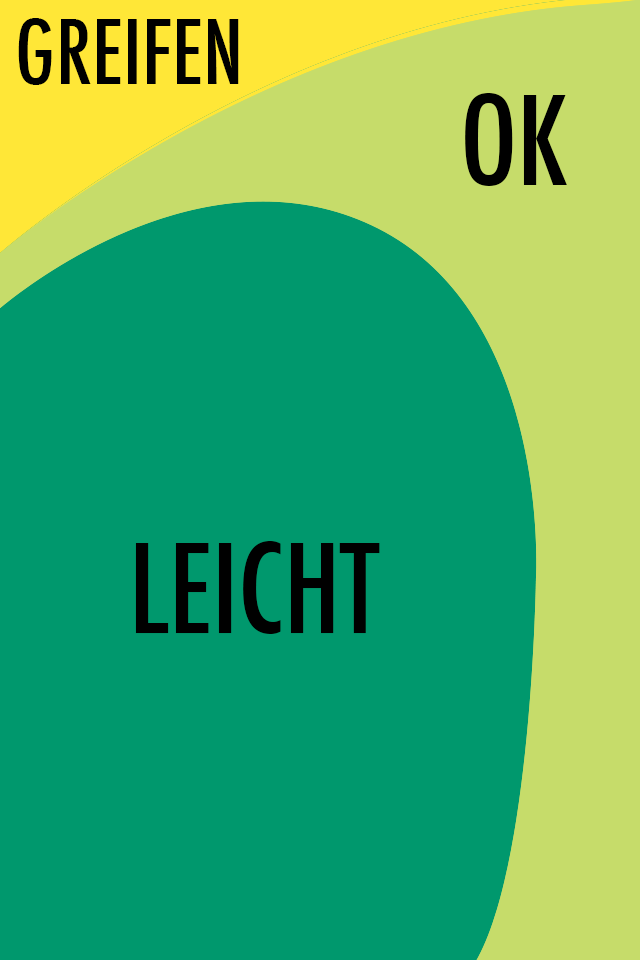
\includegraphics[width=1\textwidth]{img/anordungDerElementeSimple.png}
			\caption{Für Rechtshänder}\label{fig:rechtsPositioning}
			
	\end{subfigure}
	\begin{subfigure}[b]{0.3\textwidth}
		\centering
			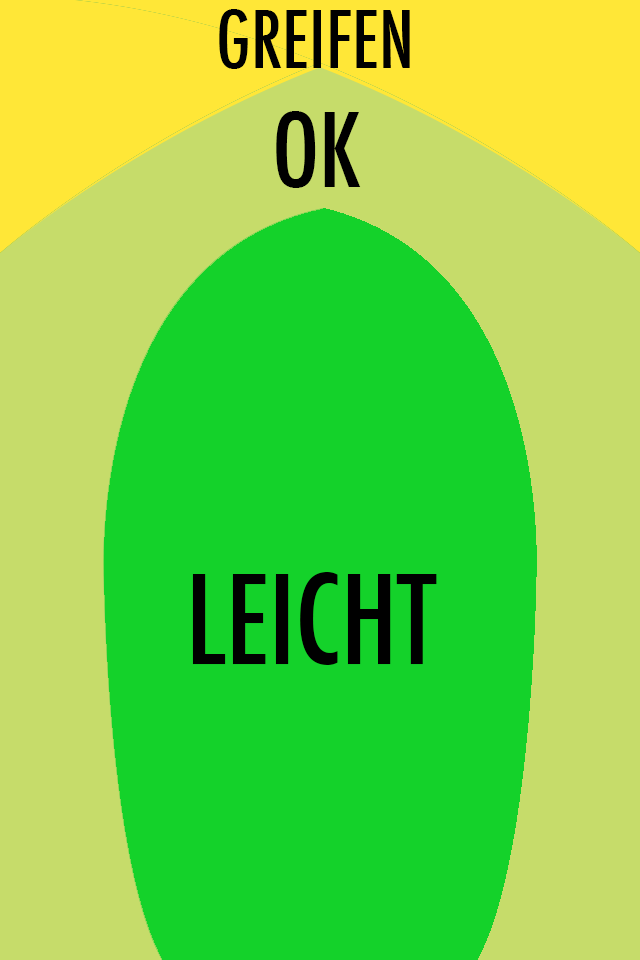
\includegraphics[width=1\textwidth]{img/anordungDerElementeForAll.png}
			\caption{Für beide Benutzergruppen}\label{fig:forallPositioning}
			
	\end{subfigure}
	\caption{Positionierung von Elementen}\label{fig:elementPos}
\end{figure}


\subparagraph{Benutze NUI} 
\label{subp:benutze_nui}

Die meisten Touchgeräten bieten einen direkte eingabe, mit denen Naturelle Gesten möglich sind. So ist es empfehlenswert Gesten auch für interaktion mit der Applikation anzubieten. Ein schönes Beispiel beitete Yahoo sketch a search, die leider nicht mehr Angeboten wird \footnote{http://techcrunch.com/2012/01/30/yahoo-shuts-down-10-mobile-apps-says-its-going-mobile-first/ }, wie in FIGURE. So konnte man den Bereich, in den man eine lokale suche machen wollte mit einen Oval zu beschränken.

Dabei muss man immer bedenken, dass in mobilen Kontext kann der benutzer nicht immer mit zwei Händen den Gerät bedienen. Somit können gesten wie Pinch, Spread oder Rotate nicht immer benutzt werden, und man sollte auf alternative Möglichkeiten zur ausführung solcher Interaktionen nachdenken. Wie in Beispiel in Figure~\ref{fig:nuibsp} Zeigt eine Oberfläche\footnote{Ausschnitt aus OpenSteetMap.com} kann man als Alternative von Pinch oder Spread Gesten, einen Schaltknopf anbieten, der eine Gleiche manipulation änlich wie mit den Gesten.

\begin{wrapfigure}{r}{0.5\textwidth}
	\begin{center}
	
	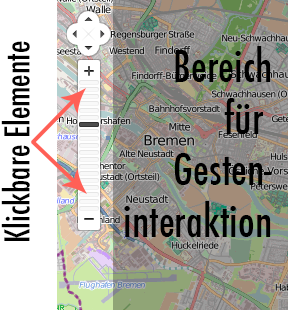
\includegraphics[width=0.3\textwidth]{img/NUIbsp.png}
	\caption{Alternative Interaktionsmöglichkeiten}\label{fig:nuibsp}
\end{center}
\end{wrapfigure}

\subparagraph{Designe für Außeneinsatz} % (fold)
\label{subp:designe_f_r_au_eneinsatz}

Design Paterns 455

\subparagraph{Gebe information in verschiedenen Ausgaben}
\label{subp:gebe_information_in_verschiedenen_ausgaben}

Notifications - LED, Alarm, etc

\subsection{Informationsaufbereitung}

- Funktionalität für mobilen kontext, seite 57 mobileFirst. In buch tapwothy sind 3 mobile behavour: micro-tasking, im local am bored. Google teilt menschen ins urgent now, repetitve now, bored now

Menschen in mobilen kontexten haben viele Wünsche und bedürfnisse die von paradigmen, die in einen stationären arbeitsplatz nicht auftauchen. Um gut benutzbare Software für solchen Szenarien zu entwicklen, ist es wichtig die Aktionen sowie Verlangen von benutzer zu wissen und zu berücksichtigen. 

Die Einteilung von Benutzer in mobilen Kontexten kann laut Google in 3 bereiche unterteilt werden: "urgent now", "repetitive now", "bored now"\cite{googleUsers}. Mit "Urgent now" ist gemeint, wenn der Benutzer Informationen ganz schnell erfahren will. Solche Informationen können sein, wie etwa die Adresse des Artzes oder Buchladens. Da diese Informationen sind Ortsabhänglig, versucht goolge die abfrage zu verbessern indem man die Benutzerort beim Abfrage hinzufügt. Bei Repretitve now ist gemeint wenn der benutzer die Gleiche art der Informationen immer wieder aufruft, wie etwa Wettervorhersage oder Aktienkursen. Bei bored now ist benutzer in zustand, wo er viel Zeit hat, etwa in emfangshalle von Flughafen, im Öffentlichen verkehrsmittel  oder Kaffe. Das Verhalten der Benutzer is dann wie von Benutzer der Stationären Rechner, aber mobile Benutzer haben nicht solche gleichen eingabe und ausgabegeräten.

Eine einteilung anhand von Interaktionstypen ist viel Detalierter und hilfreicher für den Design von Informationsaufbereitung. So können die mobile Interaktionen in vier Kategorien eingeteilt (anhand \cite[Seite 50]{mobileFirst}):

\begin{itemize}
 	\item[Suche] Ich brauche eine Antwort, sofort
 	\item[Erforschen/Spielen] Ich habe Zeit, und will eine kurze Ablenkung
 	\item[Einchecken/Status] Irgendwas ändert sich, und will ich wissen oder Teilen
 	\item[Editieren/Kreieren] Ich muss was schnell erledigen
 \end{itemize} 

Anhand diese Interaktionsparadigmen, kann man paar regeln oder hinweise für erstellung oder modifizierung von applikationen erfassen.

\subparagraph{Mach es schlank} 
\label{subp:entferne_das_fett}

Wie schon in der Einleitung von diesen Kapitel erwähnt wurde, emfehlt Jakob Nielsen die Informationsangebote auf mobilen Webseiten zu schmallern. Auch die Funktionsangebot soll zu den Mobilen Kontext passen. Als Beispiel kann hier die Amazon webseite sein (siehe Figure~\ref{fig:amazon}. So wird auf der mobile Webseite bei der Auswahl von einen Produkt, der Bild, preis und sofortige Kaufen oder Merken angeboten. In vergleich zu eine normale Webseite ist hier die Information nicht auf einmal angeboten, sondern ist viel kleiner(siehe Figure~\ref{fig:amazonFull}). Detalierte Informationen, die aber auch nur teil von normalen Webseiten beinhalten, können bei Bedarf ausgewählt werden. 

\begin{figure}
	\centering
	\begin{subfigure}[b]{0.3\textwidth}
		\centering
		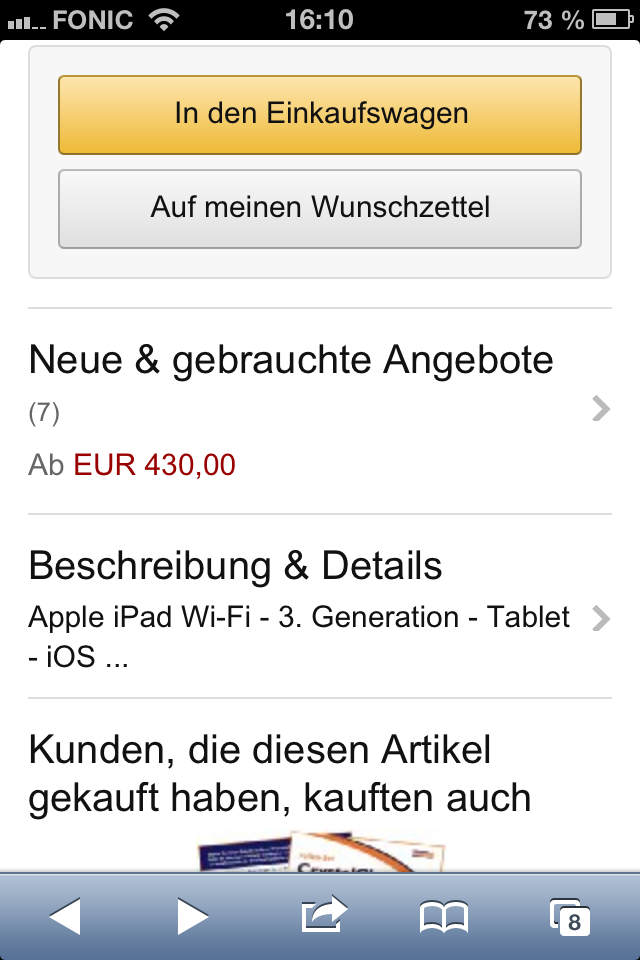
\includegraphics[width=1\textwidth]{img/amazon.png}
		\caption{Mobile Webseite}\label{fig:amazon}
	\end{subfigure}
	\begin{subfigure}[b]{0.6\textwidth}
		\centering
		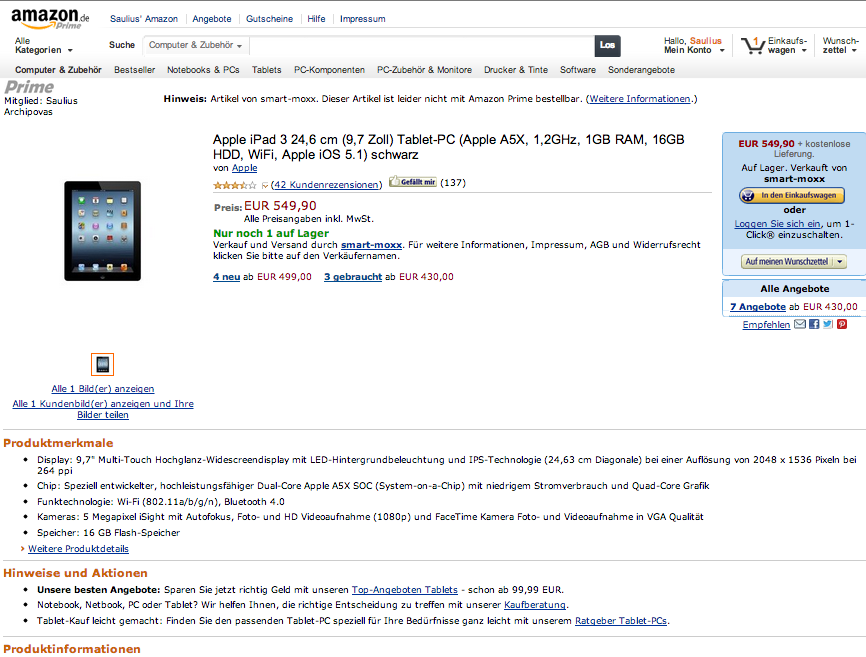
\includegraphics[width=1\textwidth]{img/amazonFull.png}
		\caption{Normale Webseite}\label{fig:amazonFull}
	\end{subfigure}
	\caption{Webseiten von Amazon}\label{fig:amazonSites}
\end{figure}

Auch mehr der Inhalt und nicht die navigation sollte in mobilen Kontext bevorzugt werden\cite[Seite 52]{mobileFirst}. So hat der Besucher der Kategorie "Erforschen/Spielen" vieleicht ein wenig Zeit um Inhalt zu konsumieren, und er sollte nicht mit eine Sitemap überfordert werden, oder überlegen wo er jetzt hin soll. So bietet etwa Youtube einen direkten Einstieg für Konsum, in den es schon Videos für den benutzer vorschlägt (siehe Figure~\ref{fig:youtube})

\begin{wrapfigure}{r}{0.5\textwidth}
	\begin{center}
	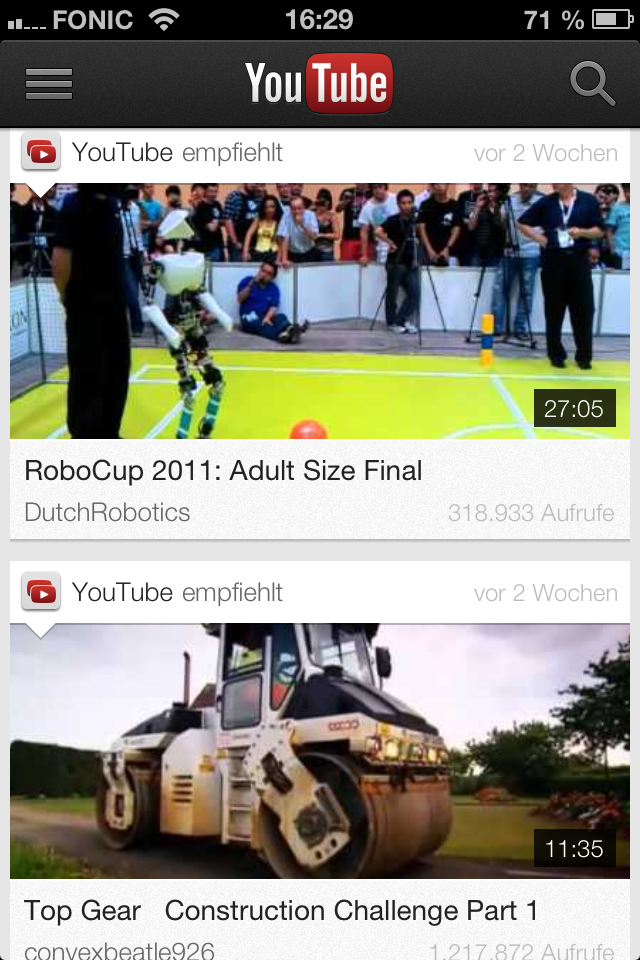
\includegraphics[width=0.3\textwidth]{img/youtube.png}
	\caption{Youtube}\label{fig:youtube}
\end{center}
\end{wrapfigure}


% Eine reduzierung der Informationsdichte kann behilflich sein, schnell auf Wichtige information zuzugreifen und somit auch die Zeit für erledigung der gewüschte aufgabe zu kürzen. So sollten nicht alle Möglichkeiten angeboten werden, sondern für die schnellen Zugriff und Erledigung ausgelegt werden. So sollte man auch die Funktionalitäten, die in Mobilen Kontext schwer zu verbeiten sind, nicht angeboten werden. Als beispiel, wäre etwa eine webseite von Amazon. 

% Wie in der Einführung erwähnt wurde, hat der Benutzer im mobilen Kontext eine kurze Zeitspanne, in der er sich auf den mobilen Gerät konzentrieren kann. So kann zu viel Funktionalität den Benutzer mehr stöhren als helfen. So ist es ratsam die wichtigen funktionaliät anzubieten, sowie die Informationsdichte zu schmalen. (cite mobileFrontier)

\subparagraph{Schneller Zugriff auf Wichtige informationen} 
\label{subp:subparagraph_name}

Wie im szenario "Suche", will der Benutzer nicht immer in das innenleben von Programmen eintauchen, nur um kleine wichtige Bruchteil der Information zu gewinnen. Deshalb sollte man wichtige Informationen schon etwa beim einem Streifblick erkenbar sein(vgl. \cite[Seite 54]{mobileFrontier} und \cite{Neil:2012uf}),  wie etwa bei iPhone Homescreen. So kann man die Piktograme so gestalten, dass sie Information selbst beinhalten, wie etwa die Piktorgram von iOS Kalender, siehe Beispiel Figure~\ref{fig:iconIos}. Auch eine Kleine Piktogram auf Piktogram kann benutzer Hinweise auf neuen Inhalt anbieten.

\begin{wrapfigure}{r}{0.5\textwidth}
	\begin{center}
	
	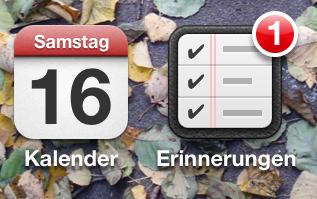
\includegraphics[width=0.3\textwidth]{img/iconIos.png}
	\caption{Schneller Zugriff auf Informationen}\label{fig:iconIos}
\end{center}
\end{wrapfigure}

% Als Beispiel dient hier der Springboard Muster\cite[Seite 3]{designPatterns},.Auch die Facebook App bedient sich an diesen muster (screenShot). Für Informationen, die Leistungen oder Ergebniss darstellen, kann man mithilfe eines Dashboard Musters erste Einstieg für Navigation gewähren. Dieses Muster ist sehr hilfreich für Analytische Applikationen.

\subparagraph{Reduziere Kognitive Aufgaben } 
\label{subp:reduziere_kognitive_aufgaben_}

In den Mobilen Kontext ist der Benutzer meistens mit verschiedene Aufgaben beschäftigt, so ist auch die verfügbarkeit der Aufmerksamkeit viel weniger, als etwa in büro. Bei Gestaltung von Applikationen, die in mobilen Kontexten dies muss immer berücksichtigt werden. So soll Anwendungen etstehen, die das unnötige Denken abnimmt. Auch die Benutzeroberfläche muss den Benutzer nicht überfordern. So sind unnötige Animationen in eine Anwendung sind ungünstig, da sie den Anwender unnötig ablenken können. Diese Bruchteile von Sekunden, die für solche Animationen in den moment gelenkt werden, werden unnötig verbraucht, da die zu erledigende Aufgabe selbst nur paar Sekunden dauern muss. Außerdem Aufgaben, die den benutzer zu viel Aufmerksamkeit verbrauchen, können auch den Benutzer gefährden, etwa wenn er viel zu abgelenkt wird bei gehen (vgl. \cite{Nasar:2008cc})



\subparagraph{Reduziere Tiefe} 
\label{subp:reduziere_das_w_hlen}

Die Herarchische Navigation ist ein viel benutzes Navigationsmuster in Applikations. So sind auch in mobilen Kontexten solche navigation übernommen. Dabei, wie auch bei den Emfehlungen in "Mach es schlank", muss man auch die Hierarchietiefe nichts zu groß halten. Mit jede weitere Tiefe muss der benutzer sich mehr Errinern und Abrufen und auch. Es wurde beobachtet bei nicht mobilen Kontexten, dass solche Navigationen eine Fehleranfähligkeit von 4\% auf 34.0\% bekommt, wenn die Navigationsstruktur von 1 bis 6 erhöht wird (Snowberry at al. Zitiert von \cite{Chae:2004gp}). Man muss auch nicht vergessen, dass der Benutzer nicht nur leichter Abgelenk wird (vgl. \cite{Oulasvirta:2005vn}), was auch eine beeinflussung auf der erfolgreiche Navigation hat.

\subparagraph{Nutze alternative Ein- und Ausgabequellen}
\label{subp:nutze_alternative_eingabenger_ten}

Die Interaktion mit den Mobilen Gerät kann in einem Mobilen Kontext durch vieles beeinflußt werden. So kann der Benutzer etwa beim Fahren einen Autos nicht mit der Hand bedient werden, oder der Blick kann nicht immer auf den Bildschirm ausgerichtet werden. So sollen auch andere Ein- oder Ausgabequellen benutzt werden. Hier bietet sich die Sprache als Ein- und Ausgabemedium.
Auch die Geolokalisierung kann sehr behilflich sein, um etwa Benutzer Informationen anzubieten bei erreichen eines Bestimmten Ortes, ohne Bewusste Eingabe des Ortes durch den Benutzer . Geolokalisierung kann auch Benutzer helfen, weniger Informationen für eine Suche anzugeben, wenn etwa er nach eine Kaffe sucht. So können schon in voraus Kaffes in Unmittelbare nähe gesucht werden.Die Benutzung von Status-Led oder Vibration kann Benutzer auf erreignisse Hinweisen, ohne dass er Immer auf den Bildschirm es sehen muss. So kann man in Android Notifications benutzen, um etwa die Status-LED mit bestimmte Farbe und Interwallen blinken zu lassen (vgl. \cite{androidNotApi}).

Es gibt aber auch eine Nachteile für Alternative Ausgaben. Es kann passieren, dass zuviele und unnötige Benachrichtigugen den Benutzer mehr Hindern als Helfen bei der Erfühlung der täglichen Aufgaben. Eine vorsichte und grundlich Nachgedachte Benutzung von alternativen Ein- und Ausgabequellen ist hier sehr geboten.

\subparagraph{Ermögliche eine Fortsetzung}
\label{subp:erm_gliche_eine_fortsetzung}

Im mobilen Kontexten wird der Benutzer oft unterbrochen in seine Aufgaben oder er hat nicht viel Zeit seine Aufgaben zu beenden. So sollen auch die Anwendungen möglichkeiten bieten die Aufgaben später zu Erledigen. Als Beispiel dient etwa der dienst Pocket. So kann man 

- In mobilen kontext wird man ständig unterbrochen
- Ausfühlen von Formularen, 

Read it later beispiele, mobileFirst seite 27

\subparagraph{Benutze Zeit fürs Ordnen}
\label{subp:benutze_zeit_als_ordnungsprinzip}


\subparagraph{Designe für Unterbrechungen} % (fold)
\label{subp:designe_f_r_unterbrechungen}


\subparagraph{Fokussiere auf Erfahrungen, die nur mobil auftreten können} % (fold)
\label{subp:fokussiere_auf_erfahrungen_die_nur_mobil_auftreten_k_nnen}

\subparagraph{Gestalte für mobilen Kontext}
\label{subp:gestalte_f_r_mobilen_kontext}



man muss auch den kontent anpassen, an den bedürfniss, seite 72 mobileFirst


\subsection{Gestaltung von Diensten}
\label{sub:gestaltung_von_diensten}

- Hier ab seite 90 (mobileFrontier) paar stichpunkte nehmen. Ist aber mehr von presi http://www.slideshare.net/preciousforever/patterns-for-multiscreen-strategies abgeleitet. 

Themen: Wechsel zwichen Geräten, da man immer im bewegung ist. So sollen Dienste gerätewechsel unterstützen. Auch die aufgaben, die man erledigt, sollten auf anderen gerät oder ort weiterzzführbar sein.

Dienste sollen auch so angepasst werden, dass die im Kernaufgaben auf beliebigen gerät laufen können.

Man sollte auch dabei aufpassen, dass man mit eine Symbiose von geräten vorhanden sein sollte. Wie etwa dass man mit einen iPhone einen Fernseher steuern kann. Also anhand des Kontextes und Ortes dienste angeboten werden sollten

\subparagraph{Dienstkoherenz und Synchronisation}
\label{subp:diensmobilit_t}

Beispiel: Evernote

- Erreichung von diesnten von beliebigen gerät.


\subparagraph{Gerätemobilität} 
\label{subp:ger_temobilit_t}

- Gerätemobilität: Benutzung von diensten in Jeden gerät. 



\subsection{Wearable Computers} 
\label{sub:wearable_computers}

- Kurze einführung, bedienung. HUD und Google Glasses

- Wichtige sachen, wo man aufpassen sollte bei der Entwicklung von GUIs für kleine bildshirme

- Probleme beim Wearable COmputers, etwa attention fragmentation
